\section{Classifier Evaluation}
\subsection{Confusion Matrix (Model Evaluation)}
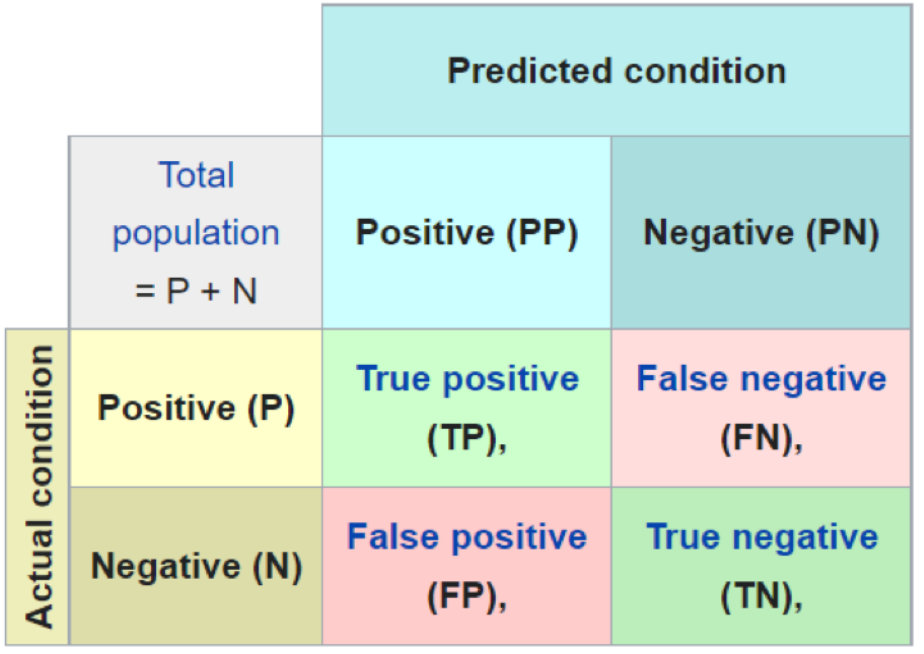
\includegraphics[width=\linewidth]{confusion-matrix.png}
\textbf{Mean Accuracy:}\\
How often is the classifier correct?\\
$Accuracy = (t_p + t_n) / n$\\
\textbf{Mean Error:}\\
How often is the classifier wrong?\\
$Error = (f_p + f_n / n)$\\
\textbf{Precision:}\\
When the prediction is 1, how often is it correct?\\
$Precision = t_p / (t_p + f_p)$\\
\textbf{Sensitivity, Recall, True Positive Rate (TPR):}\\
How often the prediction is 1, when it's actually 1?\\
$Recall = t_p / (t_p + f_n)$\\
\textbf{False Positive Rate (FPR):}\\
How often the prediction is 0, when it's actually 0?\\
$FPR = f_p / (f_p + t_n)$\\
\textbf{Miss Rate, False Negative Rate (FNR):}\\
$Miss Rate = 1 - TPR$

\subsection{Mean Accuracy}
Can be misleading. If you guess 100\% of Applicants are denied, and actually 90\% are really denied, accuracy is 90\%.
But the precision and recall are bad.\\
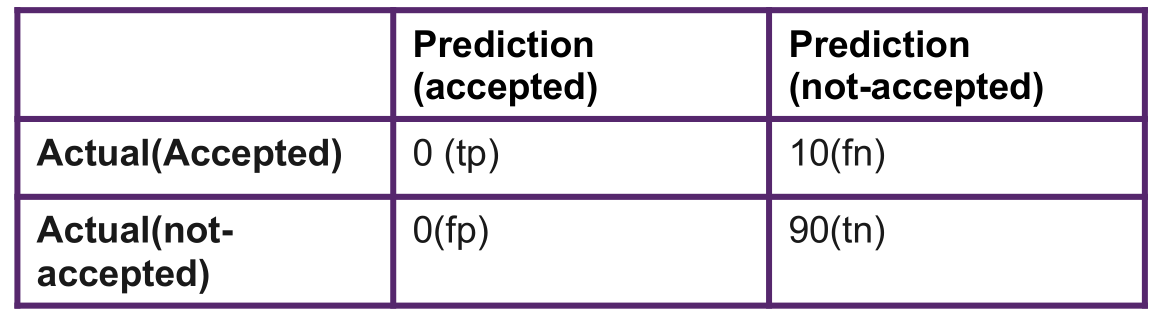
\includegraphics[width=\linewidth]{accuracy-problem.png}\\
$Precision = \frac{0}{(0 + 0)} = \frac{0}{0}$\\
$Recall = \frac{0}{(0 + 10)} = 0$

\subsection{Precision vs. Recall Tradeoff}
Increasing precision reduces recall and vice versa.\\
\textbf{Example 1} - classify safe videos for kids:
\begin{itemize}
  \item Low recall (rejects many safe videos), i.e., high precision (keeps only safe ones)
  \item High recall (rejects few safe videos), i.e., low precision (keeps unsafe videos)
\end{itemize}
\textbf{Example 2} - classify shoplifters:
\begin{itemize}
  \item Low precision but High recall ( false alerts are ok)
\end{itemize}

\subsection{Where to set the Threshold?}
It's a business decision. Rather have high precision or high recall.

\subsubsection{Precision vs. Recall Curve}
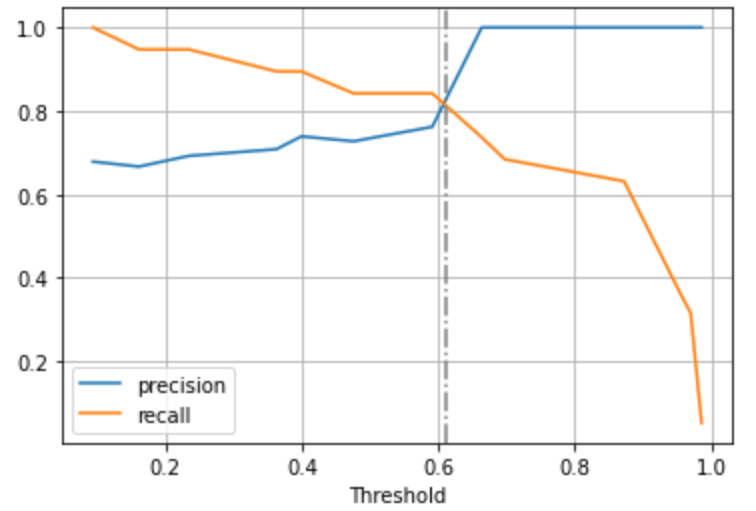
\includegraphics[width=\linewidth]{precision-recall-curve.png}

\subsubsection{Receiver Operating Characteristics (ROC)}
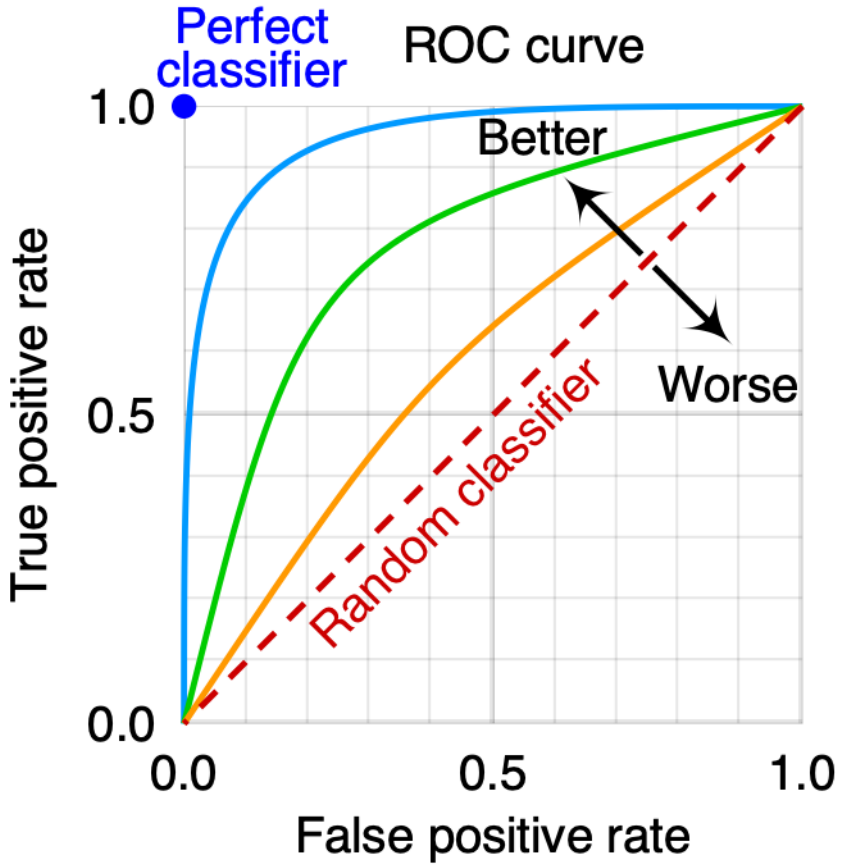
\includegraphics[width=0.7\linewidth]{roc.png}\\
Depicts relative trade-offs between true positive (benefits) and false positive (costs).\\
\textbf{AUC:} Area under (ROC) curve. 
The greater the area under the curve, shows the higher quality of the model.
Model has to be trained \textbf{multiple} times, to create a curve. One time is only a point.
